\begin{frame}{\lstinline{pystencils}}
\begin{columns}
  \column{0.58\linewidth}
  \begin{outline}
  \1 Introduced in \cite{Bauer2019} (2019)
  \1 Stencil Compiler 
  \2 Generate C or CUDA source
  \2 \lstinline{sympy} based IR
  \2 Assignments + Instructions
  \2 Static Single Assignment (SSA)
  \1 Kernels can be
  \2 Compiled and used with \lstinline{numpy}
  \2 Integrated with other code (e.g. waLBerla)
  \end{outline}

  \column{0.38\linewidth}
  \centering
  \begin{center}
    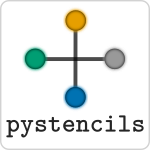
\includegraphics[width=2cm]{pystencils_logo.png}

    \vspace{1cm}

    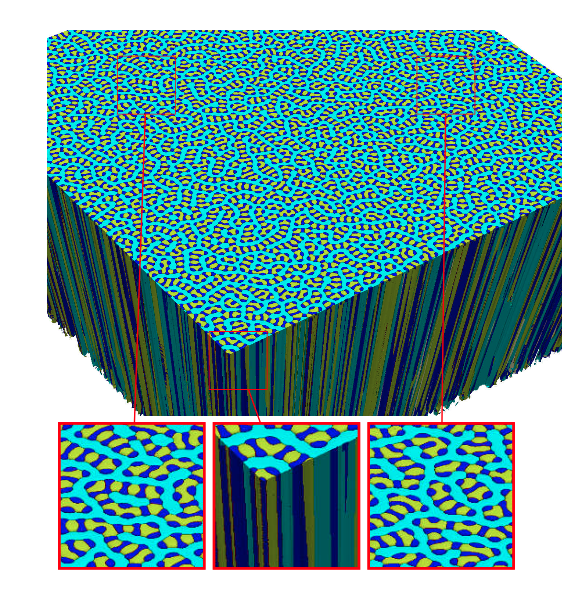
\includegraphics[width=3cm]{phase_field.png}
  \end{center}
\end{columns}
\blfootnote{From \cite{Bauer2019}}
\end{frame}
